\documentclass[10pt,letterpaper]{article}
\usepackage[utf8]{inputenc}
\usepackage{amsmath}
\usepackage{amsfonts}
\usepackage{amssymb}
\usepackage{makeidx}
\usepackage{graphicx}
\usepackage{float}
\usepackage{svg}
\usepackage{pgfplots}
\usepackage{subcaption}
\usepackage{fancyhdr}
\usepackage{float}
\usepackage{tikz}
\usepackage{nth}
\usepackage{multicol}
\usepackage{siunitx}
\usepackage[margin=1in]{geometry}

% Custom commands
\newcommand{\ts}{\textsubscript}

% Page semantics
\pagestyle{fancy}
\fancyhead[L]{\slshape\MakeUppercase{APSC 210}}
\fancyhead[R]{\slshape Muchen He}
\fancyfoot{}
\fancyfoot[C]{\thepage}

\parindent 0ex

% Meta
\author{Muchen He}
\title{APSC 210 Work Term Report}
\begin{document}
\begin{titlepage}
	\begin{center}
		\vspace*{3in}
		\line(1, 0){400}\\
		\Huge{\textbf{Game Dev @ BioWare}}\\[0.2cm]
		\large{\textbf{Career Development Report (Work Term 2)}}\\[1cm]
		\Large{\textbf{APSC 210}}\\
		\textbf{University of British Columbia}\\
		\line(1, 0){400}\\
		\vfill
		\Large{Muchen He}\\
		\large{Associate Developer, BioWare Edmonton}\\
		44638154\\

		\today \\
	\end{center}
\end{titlepage}

% Table of contents
\setcounter{secnumdepth}{3}
\tableofcontents
\thispagestyle{empty}
\clearpage

% list of tables and figures
\thispagestyle{empty}
\listoffigures
\listoftables
\newpage

\setcounter{page}{1}
\setcounter{section}{-1}

% Starting of report content
\section{Introduction}\label{introduction}

\subsection{Outline}\label{introduction-outline}

This report serves to probe the progression of career development. This report is written with intent to achieve helping us gauge our current desired career path by reviewing the skills obtained throughout the work term, as well as future desired skills that would be necessary for future careers. \\
\\
The report is broken down into four parts to help us understand what is it we need to proceed in our career development: industry in current work term, current skills being obtained, desired future industry, and transferable skills that might aid us reaching there.\\
\\
The report will also briefly describe the company and the industry it takes position in. The studio that I work for is BioWare, which is a subsidiary of a larger publisher, Electronic Arts (EA).

\subsection{Scope}\label{introduction-scope}

The scope of report consists of analysis of skills and duty pertained to me and future desired skills. The report will not include details about the game, engine, or other technology used during the work term that helped me obtaining skills or reach my objectives.

\subsection{Industry}\label{introduction-industry}

EA or BioWare, like many other studios or publishers exist in the market right now  falls into the consumer entertainment industry. The products produced is associated with Microsoft and Sony as they develop the hardware the games will run on. Future industries I wish to work in consist of electronics development or robotics and control systems.\\
\\
\textit{Work Term Industry} (section \ref{work-term-industry}) provides insight the industry with which we are currently working and competing in. This section outlines the company's position and its competitions in the gaming and or online entertainment and content delivery industry.

\subsection{Company}\label{introduction-company}

BioWare is founded in 1995, is a video game studio in Edmonton, AB. Now it is a division of Electronic Arts (EA). The studio is infamous for its story-driven games with rich, branched quests including franchises such as Mass Effect and Dragon Age \cite{bioware} \cite{bioware-wiki} \cite{bioware-wiki-list}.\\
\\
There is a pipeline of games the studio outputs, the latest one being Anthem, showcased at the Electronic Entertainment Expo (E3) in 2017 and 2018. The game so far has won many E3 awards.\\
\\
My position is an associate developer on the UI/UX team for the game Anthem. Mostly developing engine tools, and elements the scriptwriters and artists can then use to add feature into the game. \\


\section{Work Term Industry}\label{work-term-industry}

% Unorganized
The "root" industry is consumer entertainment. This includes games, TV shows, movies, sports, etc. It is to be noted that even though the BioWare studio develops games, the publisher is associated with franchises in films such as Star Wars and sports such as NHL, NBA, Madden, etc.\\
\\
The more specific work term industry this belongs to is the ``video game industry" \cite{video-game-industry}. The industry consists of hardware development and manufacturing (such as video game consoles, controllers, computers, etc.), software (programming, servers and infrastructures), and content creation (art, videos). The following graph breaks down the roles for video game industry \cite{EA-intern-conf-2} (at least in the perspective of EA).

\begin{figure}[H]
	\centering
	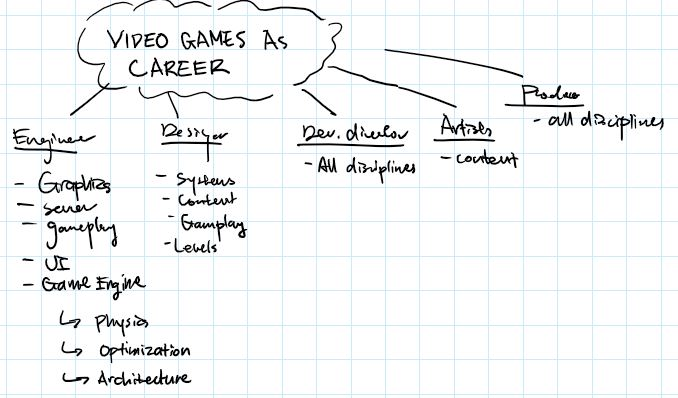
\includegraphics[width=0.6\textwidth]{assets/video-games-career-roles}
	\caption{Video game as career}
\end{figure}

One competitor in the industry, Rockstar, and their most recent products Grand Theft Auto V (GTA 5) has become the most profitable product in the industry \cite{IGN-gta5}. With a total revenue of \$6 billion, it has made "more money than any film, book, or game".
% end of unorganized

\subsection{History}

\subsection{Economic Status}

\subsection{Geographics \& Concentrations}

\subsection{Opportunities for Engineers}

\subsection{Employers in the Industry}

\subsection{Economic Factors}

\subsection{Political Factors}

\section{Obtained Skills}\label{obtained-skills}

This section provides an overview of my technical and non-technical skills gained at BioWare over the course of the work term. \\
\\

The obtained technical skills include:
- Gained more programming experience in C++
- specifically, OOP and design patters for games engines (render thread, simulation thread, UI handling)
- Gained experience in writing C\# for applications
- Increased learning skill of using propriatery engine editor
- Visual scripting
- Use python to write upgrade script for game assets
- Understood the structure and serialization of these assets, as well as the entities and links within
- Use enterprise level version control Perforce
- Work with packages and modules that are separated from the game codebase
- Agile methodologies including code review, creating and resolving JIRA tasks
- Contributing to the documentation (confluence, wiki, etc)
- Improved debugging skills in Visual Studio
- Writing code that complies with coding standard

Social skills:
- Asking for help from anyone in the office
- Participating in design review

\section{Desired Future Industry}\label{desired-future-industry}

% TODO: encapsulate the desired industries into items provided in the handbook

I have three options:

1. (Depth)
- Continue down the software development path on UI/UX or app development. Although drifted from area of study, could be a viable option to consolidate existing skills and experiences

Possible industries:
- Software development (Microsoft, Google, Startups)
- Video game industy (Coming back to EA or other game publishers)

Benefits:
- Already know a lot of things
- Easier integration and on boarding for future opportunities

Tradeoffs:
- The experiences and skills in this particular area snowballs: because the more experiences I have as software developer, the more likely I would get a position that is software developer in the future
- Not very hands on, sometimes could get very abstract => lss personal satisfaction.

2. (Breadth)
- Try something else to expand my set of skills to different areas.
- Include and apply knowledge more related to area of study (electronics, mechanical, controls, robotics, PCB, etc)

Possible industries:
- Electronics and hardware (Intel, etc)
- Robotics or control systems

Benefits:
- Experience new things, gain insight and additional interests
- Technical experience is not fixated on software development
- More hands on

3. (Academic or Research)
- Research positions (universites, NRC, CSA, etc.)
- Research discipline can be both computer science or research regarding electronics or control systems

Benefits:
- Research experience
- Grad school recommendations

\section{Technical \& Transferable Skills for Senior Work Terms}\label{transferable-skills}

% Unorganized
Technical communication skills
- Documentation contribution
- Coding standard

Learning Skills
- Asking for help
- Knowing how to get help
-

Social skills
- Small talks

\subsection{Self-Marketable Skills}

\subsection{Skills Required to Succeed}

\subsection{Plan to Obtain}

\section*{Conclusion}\label{conclusion}
\addcontentsline{toc}{section}{Conclusion}

\begin{thebibliography}{}
	% Bibliography

	\bibitem{bioware}
	BioWare | Rich Stories, Unforgettable Characters, And Vast Worlds. (2018). Retrieved May 23, 2018, from http://www.bioware.com/en/

	\bibitem{bioware-wiki}
	BioWare. (2018, May 23). Retrieved May 23, 2018, from https://en.wikipedia.org/wiki/BioWare

	\bibitem{bioware-wiki-list}
	List of BioWare video games. (2018, May 22). Retrieved May 23, 2018, from https://en.wikipedia.org/wiki/List\_of\_BioWare\_video\_games

	\bibitem{VG247-bf5}
	Nunneley, S. (2018, May 8). Battlefield 5 will feature "unique battles" and new challenges, Anthem to be designed around player input. VG247. Retrieved May 8, 2018, from https://www.vg247.com/2018/05/08/battlefield-5-unique-battles-challenges-anthem/

	\bibitem{IGN-gta5}
	Arif, S. (2018, April 9). GTA 5 Has Made More Money Than Any Film, Book, or Game, Says Analyst. Retrieved May 10, 2018, from http://ca.ign.com/articles/2018/04/09/gta-5-has-made-more-money-than-any-film-book-or-game-says-analyst

	\bibitem{video-game-industry}
	Video Game Industry. (2018, June 24). Retrieved June 24. 2018, from https://en.wikipedia.org/wiki/Video\_game\_industry

	\bibitem{EA-intern-conf-2}
	Some guest speaker <todo>

\end{thebibliography}

\end{document}